\documentclass[12pt]{article}
\usepackage[utf8]{inputenc}
\usepackage{graphicx}
\title{Finite State Machine}
\author{A.SAI MAHESH}
\begin{document}
\maketitle
\centering
\section{List of inputs given}
\begin{table}[h]
\centering
\begin{tabular}{|l|l|l|l|}
\hline
Signal Name & Signal Symbol & I1 & I2\\
\hline
Right & R & 0 & 1\\
\hline
Left & L & 1 & 0\\
\hline
Hazard & X & 1 & 1\\
\hline
\end{tabular}
\end{table}
\section{List of possible states}
\begin{table}[h]
\centering
\begin{tabular}{|l|l|l|p{2cm}|l|l|}
\hline
A & B & C & State Name & Q1 & Q2\\
\hline
1 & 0 & 0 & S1 & 0 & 1\\
\hline
0 & 1 & 0 & S2 & 1 & 0\\
\hline
0 & 0 & 1 & S3 & 1 & 1\\
\hline
0 & 0 & 0 & S0 & 0 & 0\\
\hline
\end{tabular}
\end{table}
\section{Number of Flip Flops used}
No. of D-Flip Flops used = 2
\section{State Transition Diagram}
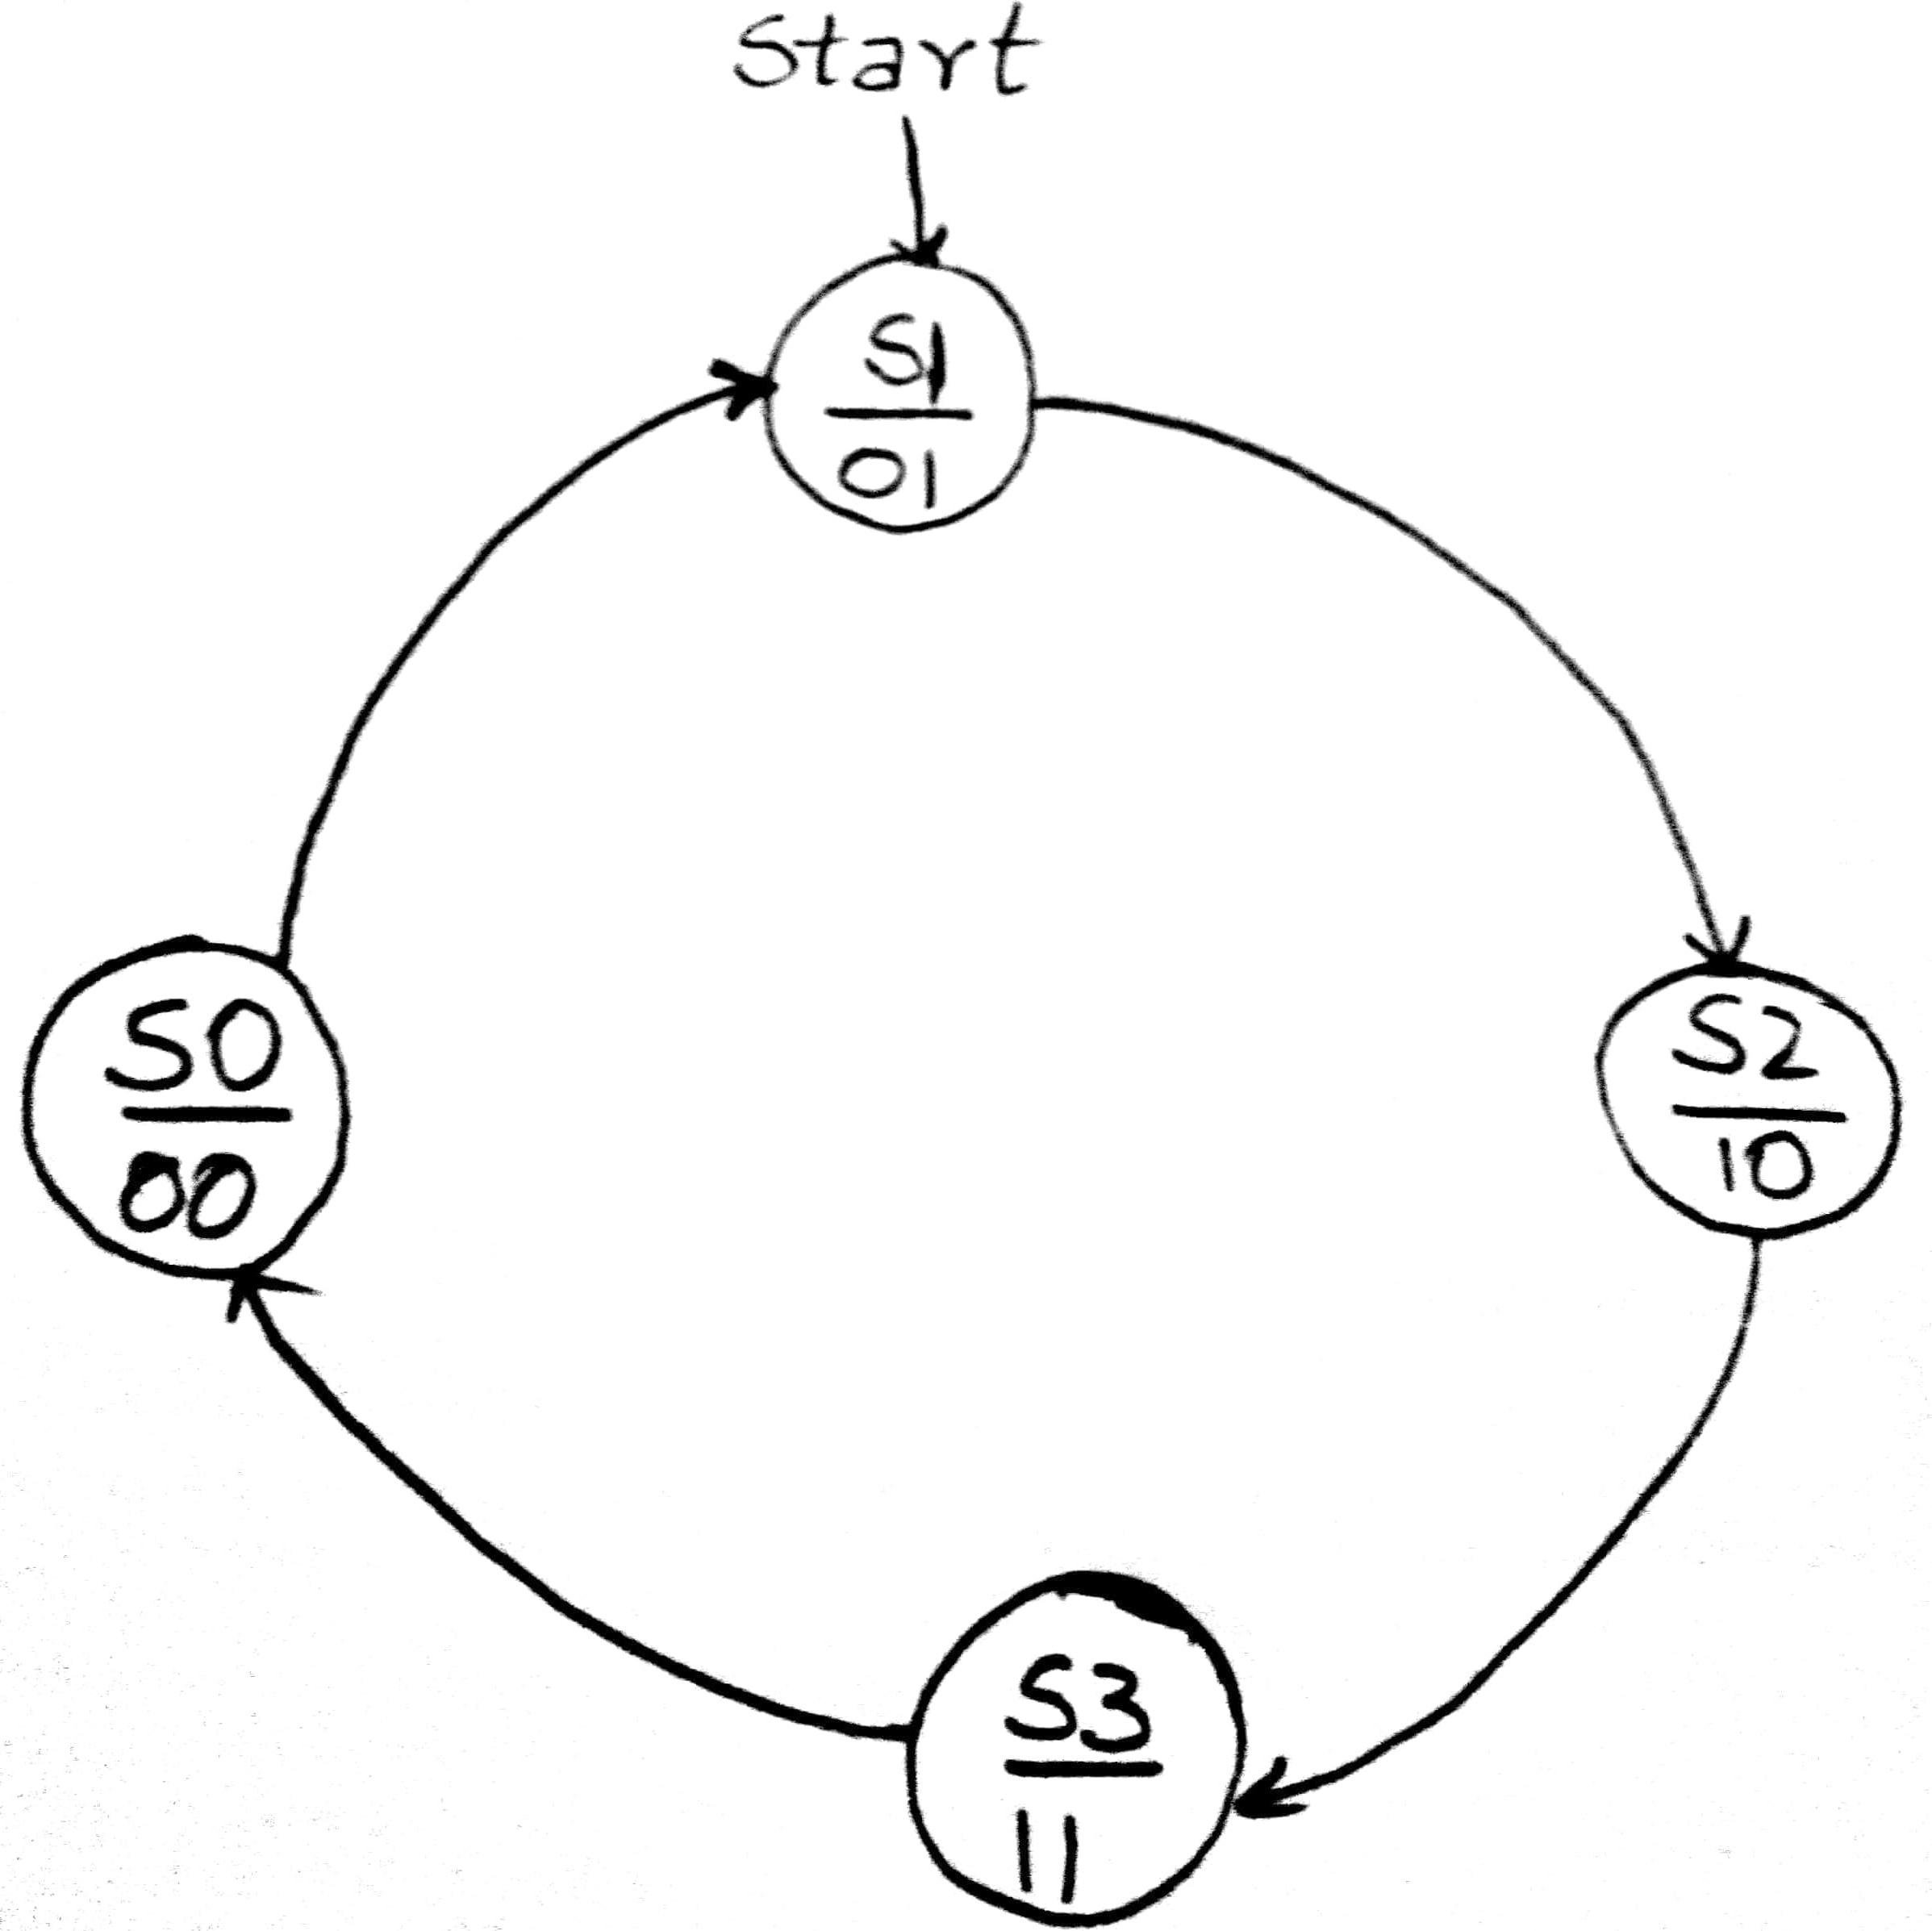
\includegraphics[width=10cm,height=10cm]{images/StateTransition.jpg}
\section{Transition Table}
\begin{table}[h]
\centering
\begin{tabular}{|c|c|c|c|}
\hline
Q1 & Q2 & D1 & D2\\
\hline
0 & 0 & 0 & 1\\
\hline
0 & 1 & 1 & 0\\
\hline
1 & 0 & 1 & 1\\
\hline
1 & 1 & 0 & 0\\
\hline
\end{tabular}
\end{table}
\section{Transition Equations of the circuit}
D1 = (Q1.!Q2)+(!Q1.Q2)

D2 = (!Q2)
\section{circuit using D flip flop}
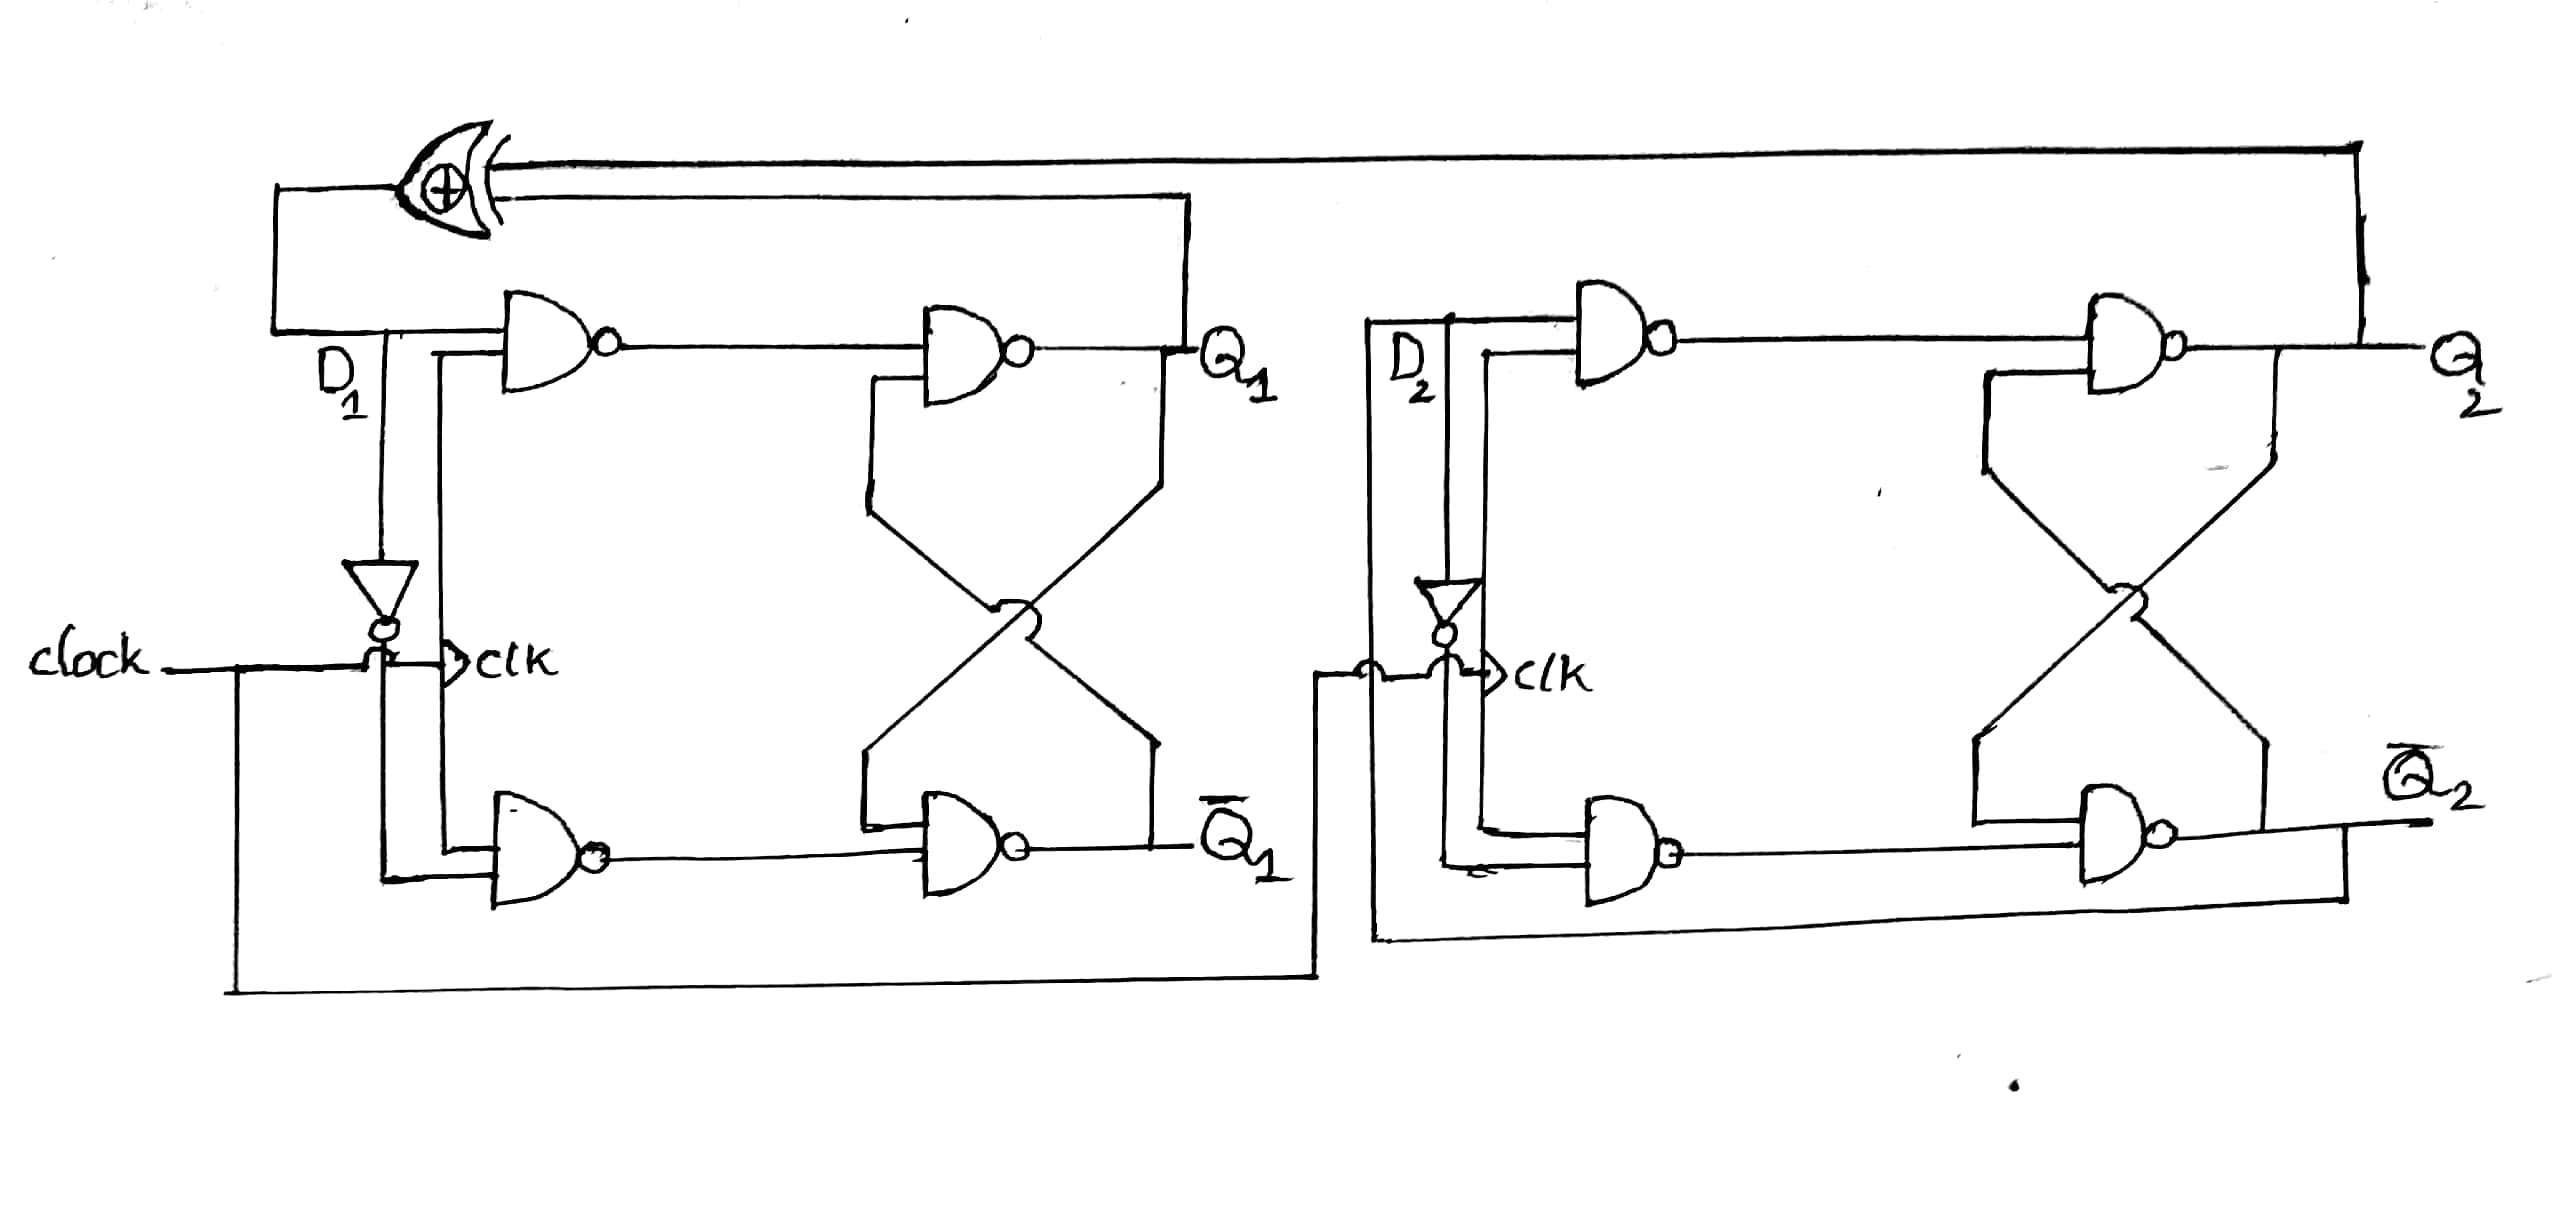
\includegraphics[width=15cm,height=10cm]{images/circuitusingdflipflop.jpg}
\end{document}